%TODO refactoring. wiecej punktów w litym tekscie 
\chapter{Automaty komórkowe}
\label{cha:Automaty komórkowe}
W rozdziale tym wyjaśniono pojęcie automatu komórkowego, przedstawiono formalną definicję automatów komórkowych oraz ich najczęstsze zastosowania. Podczas omawiania automatów zamieszczono ogólny algorytm symulacji z wykorzystaniem automatów komórkowych. Zasadę działania prostych automatów przedstawiono
na przykładzie gry Life. Szczególną uwagę podczas opisu 
 automatów komórkowych poświęcono niehomogenicznym automatom komórkowym, gdyż to one zostały wykorzystane
do symulacji pożaru. 
\section {Definicja automatu komórkowego}
Według definicji \textbf {Ferbera} \textsl{ Automat komórkowy jest dyskretnym, dynamicznych systemem, którego zachowanie jest
całkowicie określone w warunkach lokalnych relacji.}
Inną definicją, ukazującą automat komórkowy w matematycznym zapisie jest definicja \textbf{Weimara}, przedstawiająca
automat jako czwórkę parametrów:
\begin{Center}
\begin {equation}
\label{def_automatu}
$CellularAutomata=(L,S,N,f)$
\end {equation}
\end{Center}
gdzie
\begin{itemize}
\item L - zbiór komórek tworzących automat
\item S - zbiór stanów, które może przyjmować komórka
\item N - zbiór sąsiadów danej komórki
\item f - funkcja przejścia, która każdą komórkę ze zbioru L przeprowadza  ze stanu $S_i$ w stan $S_(i+1)$. $S_t$ jest jednym ze stanów
		ze zbioru S przyjmowanym przez komórkę w i-tej jednostce czasu, natomiast $S_(i+1)$ jest stanem przyjmowanym
		przez komórkę w i+1-ej jednostce czasu na podstawie analizy stanów sąsiadów komórki (N).
\end{itemize}
Innymi słowy, automat komórkowy jest to model matematyczny opisujący siatkę komórek, ich stany oraz reguły przejść
między kolejnymi stanami. Każda komórka z pewnej dyskretnej siatki komórek może przyjmować jeden z określonego zbioru stanów.
W dyskretnych przedziałach czasowych następuje ewolucja komórki, na podstawie jej \textbf{stanu poprzedniego} oraz \textbf{stanu jej sąsiadów}. Ewolucję komórki określa funkcja przejścia. Odpowiedni dobór zbioru stanów oraz funkcji przejść kształtuje cechy automatu, jego dynamikę oraz szybkość.
W wyniku ewolucji komórka przyjmuje kolejny stan ze zbioru S. Ze względu na wielowymiarowość automatów komórkowych, sąsiedztwa można
definiować w różny sposób. W przypadku dwuwymiarowego automatu najprostszym sąsiedztwem, zwanym też sąsiedztwem von Neumana będzie
zbiór czterech komórek {N,S,E,W} gdzie kolejne literki oznaczają kierunki zgodne z różą wiatrów. W dwuwymiarowych automacie jako sąsiedztwo można przyjmować także zbiór ośmiu komórek (sąsiedztwo \textbf{Moore'a}: cztery wspomniane powyżej kierunki wraz z kierunkami pośrednimi {N, S, E, W, NW, NE, SE, SW}. W trójwymiarowym automacie najprostszym sąsiedztwem jest zbiór wszystkich 
komórek połączonych ścianami z aktualnym sześcianem. Innym sąsiedztwem mogą być wszystkie sześciany połączone z aktualnie badanym
zarówno ścianami jak i krawędziami. Ważnymi elementami automatu komórkowego jest stan początkowy automatu, czyli z góry określony
stan każdej komórki w chwili 0 (przed pierwszą iteracją algorytmu). W przypadku automatów komórkowych o ograniczonej siatce konieczne
jest także zdefiniowanie warunków brzegowych. Warunki brzegowe określają reguły przejść dla komórek znajdujących się na brzegach
automatu. W przypadku jednowymiarowej siatki, przykładem warunku brzegowego jest określenie sąsiadów ostatniego $n-tego$ elementu jako 
$n-1$ oraz $1$ - przedostatni oraz pierwszy element.
Poniżej przedstawiono ogólny schemat działania algorytmu komórkowego: \\\\
\begin{center}
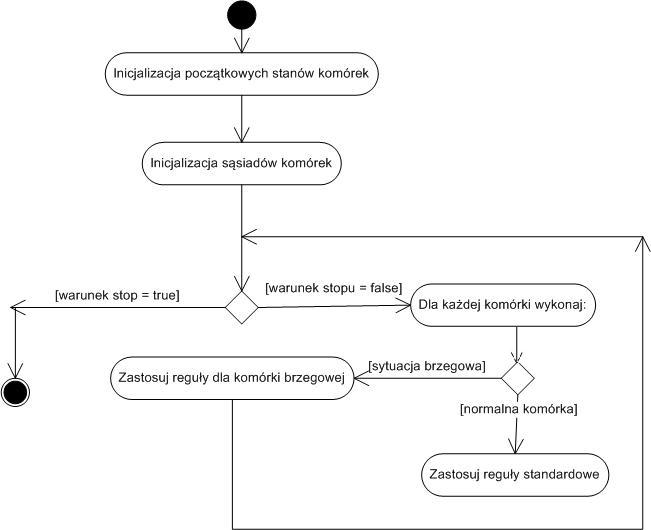
\includegraphics{algorytm_automatu_kom}
\end{center}
\\\\
Automaty komórkowe dzięki możliwościom zastąpienia bardzo skomplikowanych wzorów prostymi regułami są szeroko stosowane do modelowania
procesów fizycznych i chemicznych np. symulacje pożarów lasów, budynków, rozprzestrzenianie lekarstw w organizmie ludzkim. 
Innym zastosowaniem jest symulacja zjawisk, które ze względu na swoją naturę, w wyniku braku znajomości
dokładnych wzorów nie mogą być odzwierciedlone w sposób dokładny. Przykładem takiej symulacji jest na przykład ruch ludzi podczas ucieczki z ewakuowanego budynku.
\section{Klasyfikacja automatów komórkowych}
Od wprowadzenia pojęcia automatu komórkowego, które datuje się na lata 40-ste XX-go wieku powstały różne metody klasyfikacji automatów komórkowych. Jedną z najważniejszych jest podział ze względu na homogeniczność automatu.
\textbf{Homogenicznym automatem komórkowym} nazywamy, automat który spełnia wszystkie postulaty homogeniczności.
Należą do nich:
\begin{itemize}
\item jednakowy zbiór stanów dla każdej komórki
\item jednakowy zbiór reguł dla każdej komórki
\item stały obszar siatki automatu
\item jednakowy schemat określający sąsiadów dla każdej komórki
\item jednakowa metoda aktualizacji wszystkich komórek
\end {itemize}


Jeżeli automat nie spełnia, \textsl {któregokolwiek} z wyżej wymienionych warunków jest klasyfikowany jako \textbf {niehomogeniczny
automat komórkowy}. 

Najprostszym przykładem klasycznego, homogenicznego automatu komórkowego jest gra \textsl{Life}. 
W grze Life mamy zazwyczaj do czynienia z nieskończoną planszą Każda
z komórek siatki może przyjmować dwa stany: jest żywa lub martwa. Każda z komórek posiada ośmiu sąsiadów - są to komórki przylegające krawędziami i rogami.W grze tej wszystkie komórki zmieniają swój stan, co pewien ustalony odstęp czasu. Nowy stan komórki jest obliczany
wyłącznie na podstawie jej poprzedniego stanu oraz stanów sąsiadów. Metoda aktualizacji komórek oraz schemat określający nowy 
stan jest identyczny dla wszystkich komórek automatu. Mimo nazwy omawianej symulacji jedynym udziałem człowieka w tej grze jest
ustawienie stanu początkowego komórek.

Innymi sposobami klasyfikacji automatów komórkowych jest podział ze względu na sąsiedztwo (sąsiedztwo Moore'a oraz von Neumana), 
ze względu na wielowymiarowość planszy (jedno-,dwu-,trój-wymiarowa,...), a także ze względu na kształt pojedynczej komórki.
W jednowymiarowym automacie komórką jest odcinek, w dwuwymiarowym najprostszym wariantem jest kwadrat, a w trójwymiarowej sześcian.
Różnie między tymi automatami zostały częściowo omówione w rozdziale poprzednim.


\end {Center}
